\documentclass[11pt]{scrartcl}
\usepackage[utf8]{inputenc}
\usepackage[sexy]{evanchen} 
\usepackage{graphicx}
\graphicspath{{8 Outsource K Math/Gambar/}}

\title{Rekursi}
\author{Azzam and Akeyla}
\date{April 2024}

\begin{document}

\maketitle

\renewcommand*\contentsname{Daftar Isi}
\tableofcontents

\newpage
\section{Contoh pengaplikasian dalam soal}
\begin{enumerate}
    \item Carilah banyaknya permutasi $f$ dari $\{1,2,3,..,n\}$ yang memenuhi kondisi $$f(i) \geq i - 1,   i=1,2,3,...,n$$
        \textbf{Solusi.} Misalkan banyak permutasi $f$ dari himpunan $\{1,2,3,...,n\}$ adalah $x_n$. Tinjau $x_{n+1}$. Karena $f(n+1) \geq n$, maka $f(n + 1) = n + 1$ atau $f(n + 1) = n$.
        \begin{enumerate}
            \item Jika $f(n + 1) = n + 1$, maka permutasi $f$ dari $\{1,2,3,..,n\}$ adalah $\{1,2,3,...,n\}$ juga. Akibatnya banyak permutasi $f$ dalam kasus ini adalah $x_n$
            \item Jika $f(n + 1) = n$, maka $f(i) = n + 1$ untuk tepat satu $1 \leq i \leq n$. Tinjau bahwa untuk suatu permutasi $f$ yang memenuhi sifat ini, dengan menukar nilai $f(i)$ dari $n + 1$ menjadi $n$, didapat suatu permutasi $f$ dari $\{1,2,3,...,n\}$.
            Akibatnya, banyak permutasi $f$ di kasus ini lebih kecil dari atau sama dengan $x_n$.
            
            Tinjau pula sebaliknya,  bahwa apabila suatu permutasi $f$ dari himpunan $\{1,2,3...,n\}$ dengan $f(i) = n$ ditukar nilainya dengan $n + 1$, kemudian ditambahkan suku $n + 1$ dengan $f(n + 1) = n$, didapatkan suatu permutasi $f$ dari $\{1,2,3,..,n+1\}$ yang memenuhi kasus kedua. Maka, banyak permutasi di kasus ini lebih besar dari sama dengan $x_n$.\\
            Sehingga, banyak permutasi $f$ dalam kasus ini adalah sama dengan $x_n$.
        \end{enumerate}
        Dari kedua kasus tersebut , didapat hubungan rekursi $$x_{n+1} = 2x_n$$ dengan $x_1 = 1$. Maka, $$x_n = 2^{n-1}$$ 
    \item Seekor semut bergerak dari titik $O(0,0)$ menuju titik $A(n,1)$ di koordinat cartesius dengan $n$ bilangan asli. Jika semut tersebut hanya dapat melewati titik-titik yang dibatasi oleh persegi panjang yang dua titik bersebrangannya adalah $O$ dan $A$, dan setiap kali bergerak, ia hanya dapat memilih salah satu gerak berikut :
        \begin{enumerate}
            \item Satu langkah ke kanan
            \item Satu langkah ke atas
            \item Diagonal ke kanan bawah
        \end{enumerate}
        Ada berapa banyak cara semut tersebut bergerak dari $O$ ke $A$ ?\\
        \textbf{Solusi.} Misalkan banyak cara semut bergerak dari titik $O(0,0)$ ke titik $B_n(n,1)$ adalah $b_n$ dan banyak cara semut bergerak dari titik $O(0,0)$ ke titik $A_n(n,0)$ adalah $a_n$. Maka $a_n$ dan $b_n$ memenuhi persamaan rekursi berikut: \\
            \begin{enumerate}
                \item $b_n = b_{n-1} + a_n$
                \item $a_n = a_{n-1} + b_{n-1}$
            \end{enumerate}
        Dari sini didapatkan hubungan 
            \begin{equation*}
                \begin{split}
                    b_{n+1} & = b_n + a_{n+1}\\
                            & = 2b_n + a_n\\  
                \end{split}
            \end{equation*}
        Sehingga $$a_n = b_{n+1} - 2b_n$$
        Padahal $a_n = b_n - b_{n-1}$, sehingga
        $$b_{n+1} - 3b_n + b_{n-1} = 0, n \geq 1$$
        dengan $b_0 = 1, b_1 = 3$. Dengan menyelesaikan persamaan rekursi ini, didapat $$b_n = \dfrac{\sqrt{5}\big((3 + \sqrt{5})^{n+1} - (3 - \sqrt{5})^{n+1}\big)}{2^n \times 10}$$
\end{enumerate}
\section{Soal - soal}
\begin{enumerate}
    \item Berapa banyak cara untuk mengubini papan $2 \times 12$ dengan domino-domino (identik) $2 \times 1$ ?
    \item Berapa banyak cara untuk mengubini papan $2 \times 10$ dengan domino identik $2 \times 1$ dan/atau ubin $2 \times 2$ ?
    \item Untuk tiap $n$ bilangan asli, misalkan $a_n$ adalah banyaknya bilangan asli $n$ digit yang digitnya hanya menggunakan angka 1 dan 2 serta tidak ada dua angka 2 yang bersebelahan. Carilah nilai dari $a_{15}$.
    \item Suatu lingkaran dibagi menjadi $n$ sektor ($n \geq 1$) seperti pada gambar di bawah. Setiap sektor akan diwarnai oleh tepat salah satu dari $k$ warna berbeda ($k \geq 3$) sedemikian hingga tidak ada dua sektor bersebelahan yang berwarna sama. Carilah banyak cara pewarnaan yang mungkin untuk $n = 1, 2, 3$ dan untuk $n \geq 4$.\\
    \begin{center}
        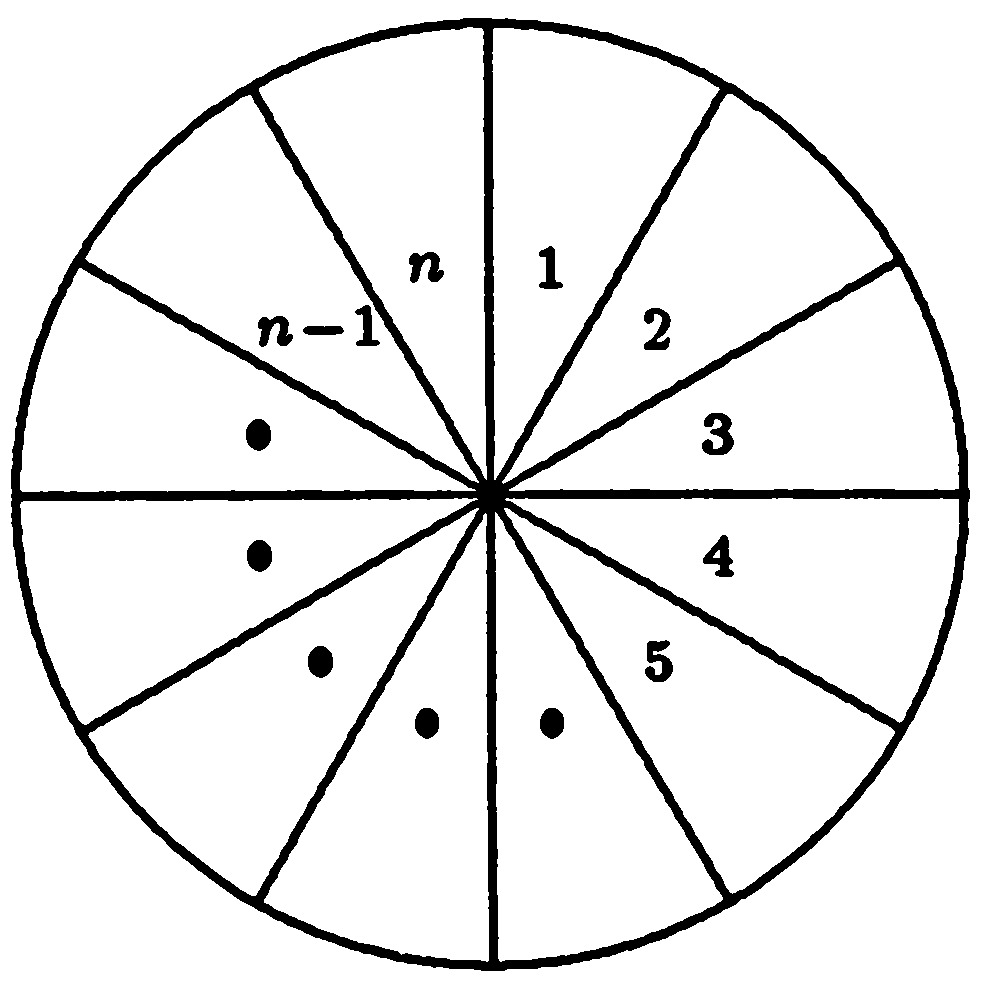
\includegraphics[width=4cm]{sector.png}
    \end{center}
    \item Di sebuah kolam, terdapat 8 batu yang membentuk segidelapan beraturan. Sebut secara berurutan batu-batu  tersebut sebagai $A, B, C, D, E, F, G$ dan $H$. Seekor katak mula-mula ada di batu $A$. Selama katak tersebut belum sampai ke batu $E$, katak tersebut akan melompat ke salah satu dari dua batu yang bersebelahan dari batu yang sedang ia tempati. Katak akan berhenti melompat begitu ia melompat ke batu $E$. Misalkan $a_n$ adalah banyak cara katak tersebut melompat sebanyak tepat $n$ kali untuk mencapai batu $E$. Buktikan bahwa $a_{2n-1} = 0$ dan $$a_{2n} = \dfrac{1}{\sqrt{2}}\{(2 + \sqrt{2})^{n-1} - (2 - \sqrt{2})^{n-1}\}$$
    \item Definisikan \textit{kata kana} sebagai string huruf yang hanya terdiri dari huruf A,B dan C sedemikian hingga tidak ada substring AB, BC, ataupun CA. Ada berapa banyak \textit{kata kana} dengan tujuh huruf?
    % \item (AIME I 2008) Definisikan \textit{kata stropik} sebagai string huruf yang hanya terdiri dari huruf A dan B sedemikian hingga setiap blok huruf A yang berurutan memiliki panjang genap sedangkan setiap blok huruf B yang berurutan memiliki panjang ganjil. Sebagai contoh, AA, B, BAABBB, AAB adalah \textit{kata stropik} sedangkan AABB, BB, BBBAABBAB bukan. Ada berapakah \textit{kata stropik} dengan panjang 14 ?
    % \item Definisikan \textit{kata na} sebagai string huruf yang hanya terdiri dari huruf A dan B sedemikian hingga tidak ada substring AAA dan BBB. Ada berapakah \textit{kata na} dengan panjang 10 ?
    \item Misalkan $f(n)$ adalah banyaknya permutasi $a_1,a_2,...,a_n$ dari $1,2,3,...,n$ sedemikian hingga 
        \begin{enumerate}
            \item $a_1 = 1$
            \item $|a_i - a_{i + 1}| \leq 2$ untuk $i = 1,2,3,...,n-1$
        \end{enumerate}
        Carilah sisa pembagian dari $f(2017) + f(2018)$ oleh 3.
\end{enumerate}
\end{document}